\documentclass[a4paper]{article}
\usepackage{amsfonts}
\usepackage{amsmath}
\usepackage{amssymb}
\usepackage{graphicx}
\begin{document}

\noindent \large Auteur: Anass Hamzaoui \\
\noindent \large Studierichting: Informatica \\
\noindent \large Oefeningenreeks 5F nr. 3.6 \\
\medskip
\normalsize

$r = 1 + 2\cos\theta$ \\

$\left|\begin{array}{ll}
    & r = 0 \implies \cos\theta = -\dfrac{1}{2} \implies \theta = \dfrac{2\pi}{3} \text{ en } \theta = -\dfrac{2\pi}{3} \\
    
    & \text{Grote lus: } \theta \in \left[-\dfrac{2\pi}{3}, \dfrac{2\pi}{3}\right] \\
    
    & \text{Kleine lus: } \theta \in \left[\dfrac{2\pi}{3}, \dfrac{4\pi}{3}\right] \\
\end{array}\right.$ \\

Grafiek: \\
\begin{figure}[h]
\centering
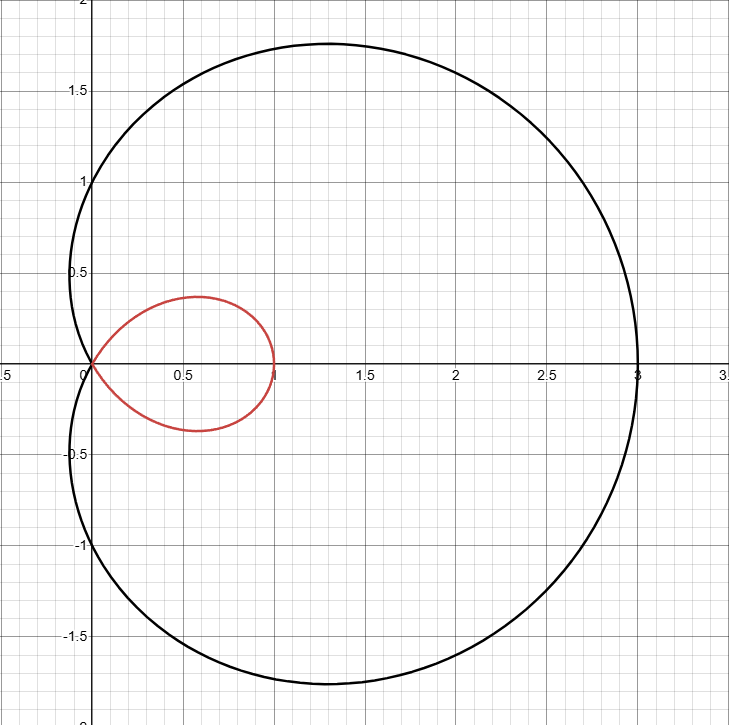
\includegraphics[width=8cm]{5F-3.6-anass.hamzaoui.INF.png}
\end{figure}

$\begin{array}{ll}
r^2 &= (1+2\cos\theta)^2 = 1 + 4\cos\theta + 4\cos^2\theta \\

&= 3 + 4\cos\theta + 2\cos 2\theta \\

\displaystyle\int r^2    d\theta &= 3\theta + 4\sin\theta + \sin 2\theta \\

S_{\text{groot}} &= \left[3\theta + 4\sin\theta + \sin 2\theta\right]_0^{2\pi/3} \\

&= 2\pi + 4\cdot\dfrac{\sqrt{3}}{2} - \dfrac{\sqrt{3}}{2} = 2\pi + \dfrac{3\sqrt{3}}{2} \\

S_{\text{klein}} &= \left[3\theta + 4\sin\theta + \sin 2\theta\right]_{2\pi/3}^{\pi} \\

&= 3\pi - \left(2\pi + \dfrac{3\sqrt{3}}{2}\right) = \pi - \dfrac{3\sqrt{3}}{2} \\

S &= S_{\text{groot}} - S_{\text{klein}} \\

&= \left(2\pi + \dfrac{3\sqrt{3}}{2}\right) - \left(\pi - \dfrac{3\sqrt{3}}{2}\right) \\

&= \pi + 3\sqrt{3} \\
\end{array}$

\begin{thebibliography}{999}
    %\bibitem{a} Referentie
\end{thebibliography}
\end{document}